%%%%%%%%%%%%%%%%%%%% chapter.tex (Chapter 4) %%%%%%%%%%%%%%%%%%%%%%%%%%%%%
% Chapter 4: Direct, Indirect & High-Radix Interconnect Topologies
%%%%%%%%%%%%%%%%%%%%%%%%%%%%%%%%%%%%%%%%%%%%%%%%%%%%%%%%%%%%%%%%%%%%%%%%%

\chapter{Direct, Indirect \& High-Radix Interconnect Topologies}
\label{ch:topologies}

\author{NoC-Lab Research Consortium}
\institute{NoC-Lab Research Consortium \at Shanghai Jiao Tong University \& International Collaborators, \email{research@network-on-chip.org}}

\maketitle

\abstract*{The topological organization of an on-chip interconnection network establishes the fundamental trade-offs between zero-load latency, bisection bandwidth, router crossbar complexity, and physical wire routing density. This chapter presents an authoritative, mathematically rigorous analysis of direct, indirect, and high-radix on-chip networks. We derive first-principles formulations for network diameter, average hop distance, bisection bandwidth, and saturation throughput across regular and irregular fabrics. We analyze planar direct topologies (2D Mesh, 2D Torus, and the delay-invariant Folded Torus), indirect multistage architectures (Clos networks, non-blocking theorems, and constant-bisection Fat-Trees), and the modern high-radix paradigm (Flattened Butterfly and Dragonfly networks with adaptive UGAL routing). Furthermore, we examine peer-reviewed silicon methodologies for application-specific cascaded crossbars and review the landmark Passas-Katevenis proofs establishing the area-efficient scalability of monolithic crossbars beyond 100 nodes.}

\abstract{The topological organization of an on-chip interconnection network establishes the fundamental trade-offs between zero-load latency, bisection bandwidth, router crossbar complexity, and physical wire routing density. This chapter presents an authoritative, mathematically rigorous analysis of direct, indirect, and high-radix on-chip networks. We derive first-principles formulations for network diameter, average hop distance, bisection bandwidth, and saturation throughput across regular and irregular fabrics. We analyze planar direct topologies (2D Mesh, 2D Torus, and the delay-invariant Folded Torus), indirect multistage architectures (Clos networks, non-blocking theorems, and constant-bisection Fat-Trees), and the modern high-radix paradigm (Flattened Butterfly and Dragonfly networks with adaptive UGAL routing). Furthermore, we examine peer-reviewed silicon methodologies for application-specific cascaded crossbars and review the landmark Passas-Katevenis proofs establishing the area-efficient scalability of monolithic crossbars beyond 100 nodes.}

\section{Interconnect Graph Theory and Formal Performance Metrics}
\label{sec:ch4_metrics}
\index{Interconnect Graph Theory}
\index{Topological Metrics}

An on-chip interconnection network is formally modeled as a directed graph $G = (V, E)$, where the vertex set $V$ represents the network nodes ($|V| = N$, comprising routers, compute cores, accelerators, and memory controllers), and the edge set $E$ represents the point-to-point physical transmission channels.

The choice of topology defines the structural limits of communication performance:
\begin{enumerate}
    \item \textbf{Router Radix ($k$)}: The number of physical input/output ports per router:
    \begin{equation}
    k = \text{deg}_{in}(u) = \text{deg}_{out}(u)
    \label{eq:ch4_radix}
    \end{equation}
    Because internal crossbar switch area and power scale quadratically ($O(k^2)$), low-radix designs minimize local switch overhead, whereas high-radix switches reduce network traversal hops at the expense of larger crossbars.
    \item \textbf{Network Diameter ($D$)}: The maximum shortest-path distance between any pair of nodes in the network:
    \begin{equation}
    D = \max_{u, v \in V} d(u, v)
    \label{eq:ch4_diameter}
    \end{equation}
    where $d(u, v)$ is the minimum hop count between $u$ and $v$. Diameter dictates worst-case communication latency.
    \item \textbf{Average Hop Distance ($\bar{h}$)}: The expected shortest-path distance under a spatial traffic probability distribution $p(u, v)$:
    \begin{equation}
    \bar{h} = \sum_{u \in V} \sum_{v \ne u} p(u, v) \cdot d(u, v)
    \label{eq:ch4_avghop}
    \end{equation}
    Under Uniform Random (UR) traffic ($p(u, v) = \frac{1}{N(N-1)}$), this reduces to $\bar{h}_{UR} = \frac{1}{N(N-1)} \sum_{u \ne v} d(u, v)$.
    \item \textbf{Bisection Bandwidth ($B_C$)}: The minimum bandwidth cut partitioning the vertex set $V$ into two equal disjoint subsets $V_1, V_2$ ($|V_1| = |V_2| = N/2$):
    \begin{equation}
    B_C = \min_{V_1, V_2} \sum_{u \in V_1, v \in V_2, (u, v) \in E} C(u, v)
    \label{eq:ch4_bisection}
    \end{equation}
    where $C(u, v)$ denotes link bandwidth. In networks with uniform channel width $W$ bits and clock frequency $f_{clk}$, bisection bandwidth is expressed as channel count $N_C$: $B_C = N_C \cdot W \cdot f_{clk}$.
    \item \textbf{Maximum Channel Load ($\gamma_{max}$) and Saturation Throughput ($\Theta_{sat}$)}:
    Let $\gamma_e$ denote the expected traffic volume traversing physical edge $e \in E$ when each node injects 1 flit per cycle. The maximum channel load is:
    \begin{equation}
    \gamma_{max} = \max_{e \in E} \gamma_e
    \label{eq:ch4_gamma}
    \end{equation}
    Because each channel can transport at most 1 flit per cycle, the theoretical maximum saturation throughput per node is bounded by:
    \begin{equation}
    \Theta_{sat} \le \frac{1}{\gamma_{max}} \le \frac{2 B_C}{N} \quad [\text{flits/node/cycle}]
    \label{eq:ch4_throughput_bound}
    \end{equation}
    \item \textbf{Zero-Load Latency ($T_0$)}: The average latency of an $L$-flit packet across uncontended routers and links:
    \begin{equation}
    T_0 = (\bar{h} + 1) \cdot t_{router} + \bar{h} \cdot t_{wire} + \left( \frac{L - 1}{\text{Rate}} \right)
    \label{eq:ch4_zero_load_lat}
    \end{equation}
\end{enumerate}

\section{Direct Topologies: Mesh, Torus, and the Folded Torus}
\label{sec:ch4_direct}
\index{2D Mesh}
\index{2D Torus}
\index{Folded Torus}

Direct topologies couple every router directly to a compute node, forming regular planar grids well-suited for standard CMOS silicon tiling.

\subsection{2D Mesh Networks}
In a $k \times k$ 2D Mesh ($N = k^2$):
\begin{itemize}
    \item \textbf{Diameter}: Opposing corners require $2(k - 1)$ hops: $D_{Mesh} = 2(k - 1)$.
    \item \textbf{Average Hop Distance}:
    \begin{equation}
    \bar{h}_{Mesh} = \frac{2}{3} k \cdot \left(1 - \frac{1}{k^2}\right) \approx \frac{2}{3} k
    \label{eq:ch4_mesh_avghop}
    \end{equation}
    \item \textbf{Bisection Bandwidth}: Bisecting the mesh cuts $k$ bidirectional links ($2k$ directional channels):
    \begin{equation}
    B_{C, Mesh} = 2k \cdot W \implies \Theta_{Mesh} \le \frac{4 W}{k}
    \label{eq:ch4_mesh_bisect}
    \end{equation}
\end{itemize}
Under uniform traffic, peripheral nodes route through the center, generating severe center-channel congestion ($\gamma_{max} \approx k/4$).

\subsection{2D Torus and the Wire Delay Dilemma}
A $k \times k$ 2D Torus ($k$-ary 2-cube) adds periodic wrap-around links. The topology becomes completely edge-symmetric:
\begin{equation}
D_{Torus} = 2 \left\lfloor \frac{k}{2} \right\rfloor, \quad \bar{h}_{Torus} \approx \frac{k}{2}, \quad B_{C, Torus} = 4k \cdot W
\label{eq:ch4_torus_metrics}
\end{equation}
A 2D Torus delivers exactly twice the bisection bandwidth and a 25\% reduction in average hop count compared to a 2D Mesh.

However, in a naive planar layout, the perimeter wrap-around wire must span the entire die:
\begin{equation}
L_{wrap} = (k - 1) \cdot L_0
\label{eq:ch4_wrap_wire}
\end{equation}
where $L_0$ is the tile pitch. By the Elmore delay model ($\tau \propto L^2$), an $8 \times 8$ torus suffers $49\times$ higher propagation delay on wrap-around wires than on local links, destroying clock frequency unless aggressively pipelined.

\subsection{The Folded Torus Invariance}
The \textbf{Folded Torus} topology solves the wrap-around wire crisis by physically interleaving even and odd nodes along each dimension:
\begin{equation}
\text{Physical Placement}: 0, \quad 2, \quad 4, \quad \dots, \quad k-2, \quad k-1, \quad \dots, \quad 3, \quad 1
\label{eq:ch4_folded_order}
\end{equation}
Every link in the Folded Torus—including all wrap-around connections—has an identical physical length:
\begin{equation}
L_{link, Folded} = 2 \cdot L_0
\label{eq:ch4_folded_len}
\end{equation}
By trading a constant wire length of $2 L_0$ for the elimination of catastrophic $(k-1) L_0$ wires, the Folded Torus achieves high clock frequencies while retaining torus bisection bandwidth and low diameter.

\section{Indirect Multistage Interconnects: Clos and Fat-Trees}
\label{sec:ch4_indirect}
\index{Clos Network}
\index{Fat-Tree}

Indirect topologies place processing elements exclusively at the network periphery, interconnecting them through intermediate switching stages.

\subsection{Clos Networks and Non-Blocking Theorems}
A 3-stage Clos network $C(n, m, r)$ comprises $r$ input switches of size $n \times m$, $m$ middle switches of size $r \times r$, and $r$ output switches of size $m \times n$~\cite{Clos1953}.
\begin{itemize}
    \item \textbf{Strictly Non-Blocking (SNB)}: Any idle input can connect to any idle output without rerouting existing calls if and only if:
    \begin{equation}
    m \ge 2n - 1
    \label{eq:ch4_clos_snb}
    \end{equation}
    \item \textbf{Rearrangeably Non-Blocking (RNB)}: By the Slepian-Duguid theorem, any input can connect to any output with potential rerouting if:
    \begin{equation}
    m \ge n
    \label{eq:ch4_clos_rnb}
    \end{equation}
\end{itemize}

\subsection{Fat-Trees and Constant Bisection Bandwidth}
Leiserson's Fat-Tree~\cite{Leiserson1985} avoids root bottlenecks by progressively increasing channel capacity toward the tree root. At each hierarchical level, the number of parallel channels doubles, preserving constant bisection bandwidth across all horizontal network partitions.

\section{High-Radix Interconnects: Flattened Butterfly and Dragonfly}
\label{sec:ch4_high_radix}
\index{High-Radix Networks}
\index{Flattened Butterfly}
\index{Dragonfly}

Modern sub-10nm CMOS technologies provide vast routing gate density, prompting a shift from low-radix/high-diameter networks to high-radix/low-diameter architectures ($k \ge 16$--$64+$).

\subsection{Flattened Butterfly}
Kim et al.~\cite{Kim2007} projected multi-stage butterfly switches into a single direct router per tile. In a $k \times k$ Flattened Butterfly, each router connects to all other routers in the same row and column:
\begin{equation}
D_{FBfly} = 2, \quad k_{radix} = 2(k - 1) + p
\label{eq:ch4_fbfly}
\end{equation}
Any node in the network is reachable in at most 2 hops, slashing router traversal cycles.

\subsection{The Dragonfly Topology and UGAL Routing}
Kim, Dally et al.~\cite{Kim2008} organized high-radix routers into local fully connected groups (cliques) interconnected by sparse global links. Under \textbf{Universal Globally-Adaptive Routing (UGAL)}, packets evaluate queuing delays: if the minimal global link is congested, packets are routed non-minimally through a randomly chosen intermediate group, eliminating hot-spot saturation.

\section{Application-Specific Synthesis \& Cascaded Crossbars}
\label{sec:ch4_application_specific}
\index{Cascaded Crossbars}
\index{Topology Synthesis}

Heterogeneous SoCs exhibit highly non-uniform communication demands. Rigid standard topologies introduce severe silicon area and power waste.

\subsection{MIRO Synthesis of Cascaded Crossbar Networks}
Jun, Yoo, and Chung~\cite{Jun2009} formulated the synthesis of cascaded crossbar switches to replace power-hungry centralized bus matrices.

\begin{figure}[htbp]
\centering
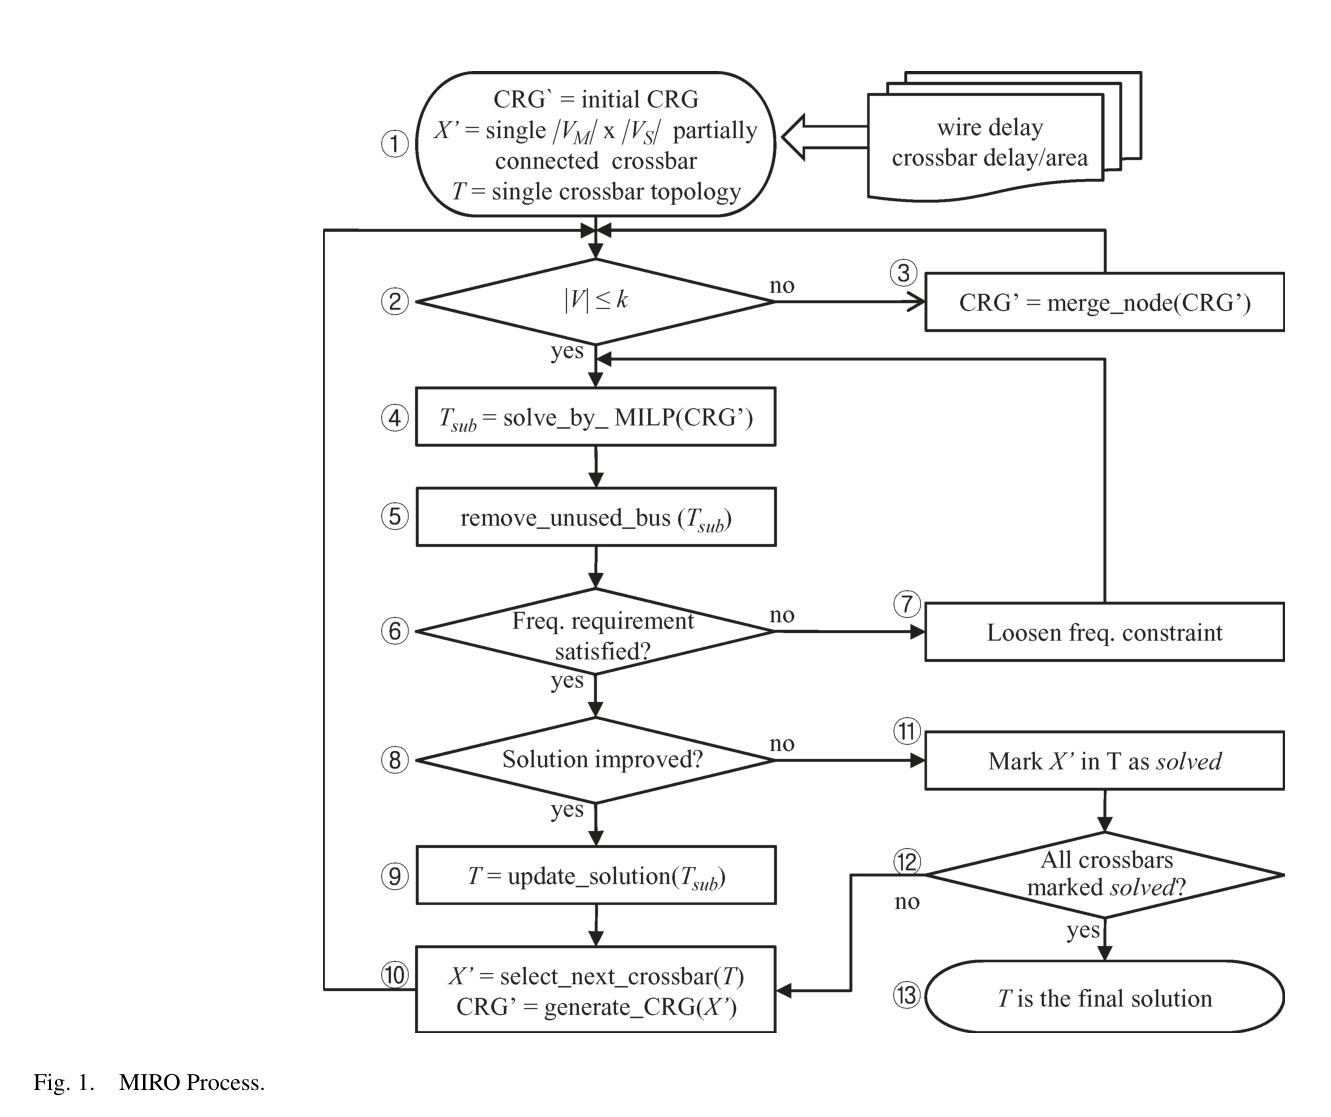
\includegraphics[width=0.75\textwidth]{chapters/ch04-topologies-and-metrics/figures/jun_fig01_miro_cascaded.png}
\caption{The MIRO (Multi-stage Interconnect Reduction and Optimization) process for synthesizing cascaded crossbar networks under bandwidth and latency constraints. [Reproduced from: M. Jun, S. Yoo, and E.-Y. Chung, ``Topology Synthesis of Cascaded Crossbar Switches,'' \emph{IEEE Trans. Comput.-Aided Design Integr. Circuits Syst.}, Vol.~28, No.~6, pp.~926--930, June 2009, DOI: 10.1109/TCAD.2009.2017079. \copyright~2009 IEEE]}
\label{fig:ch4_miro}
\end{figure}

Jun et al. proved that while Mixed Integer Linear Programming (MILP) discovers exact optimal topologies, its computational complexity explodes for $|V| > 16$. The MIRO heuristic clusters masters based on communication affinities, achieving \textbf{up to 69.5\% area reduction} over conventional architectures while satisfying all clock frequency requirements.

\subsection{Switch Merger and Partitioning Algorithms}
Dumitriu and Khan~\cite{Dumitriu2009} introduced transaction-oriented topology generation using iterative switch merging and partitioning:

\begin{figure}[htbp]
\centering
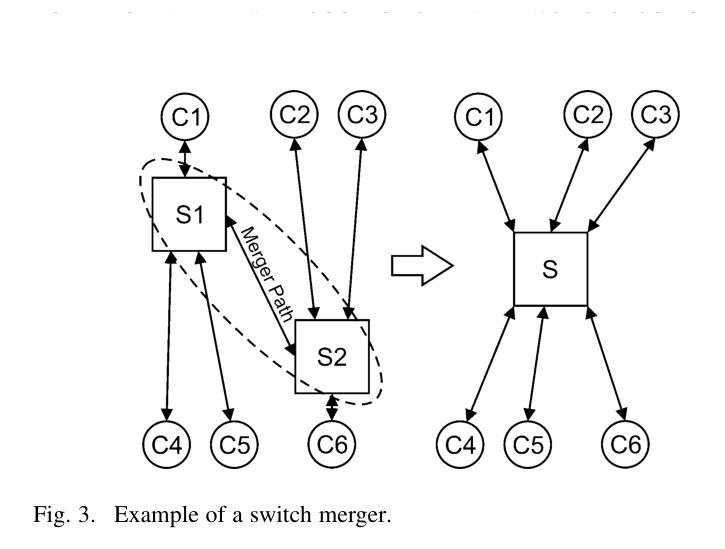
\includegraphics[width=0.48\textwidth]{chapters/ch04-topologies-and-metrics/figures/dumitriu_fig03_switch_merger.png}
\hfill
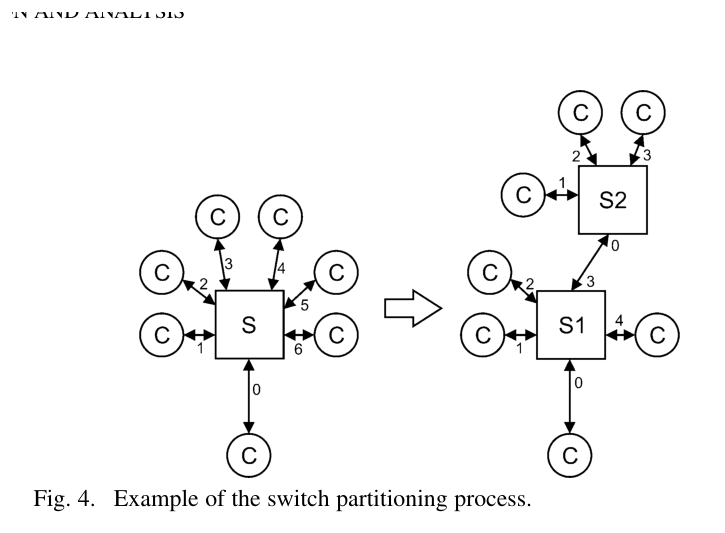
\includegraphics[width=0.48\textwidth]{chapters/ch04-topologies-and-metrics/figures/dumitriu_fig04_switch_partition.png}
\caption{Application-specific topology optimization: (left) switch merger process combining low-traffic routers; (right) switch partitioning process dividing congested routers to meet physical pin and timing constraints. [Reproduced from: V. Dumitriu and G. N. Khan, ``Throughput-Oriented NoC Topology Generation and Analysis for High Performance SoCs,'' \emph{IEEE Trans. Very Large Scale Integr. (VLSI) Syst.}, Vol.~17, No.~10, pp.~1433--1446, October 2009, DOI: 10.1109/TVLSI.2008.2006798. \copyright~2009 IEEE]}
\label{fig:ch4_dumitriu}
\end{figure}

By using predictive contention modeling during synthesis, the resulting topologies matched or exceeded regular 2D mesh throughput while utilizing \textbf{50\% fewer network resources}.

\section{Silicon Floorplanning Limits: The Passas Radix-128 Proof}
\label{sec:ch4_passas}
\index{Crossbar Scalability}

A persistent misconception in early literature asserted that full crossbar networks are unviable beyond 32 nodes. Passas, Katevenis, and Pnevmatikatos~\cite{Passas2012} refuted this by modeling and fabricating a **radix-128 crossbar in 90~nm CMOS**.

\begin{figure}[htbp]
\centering
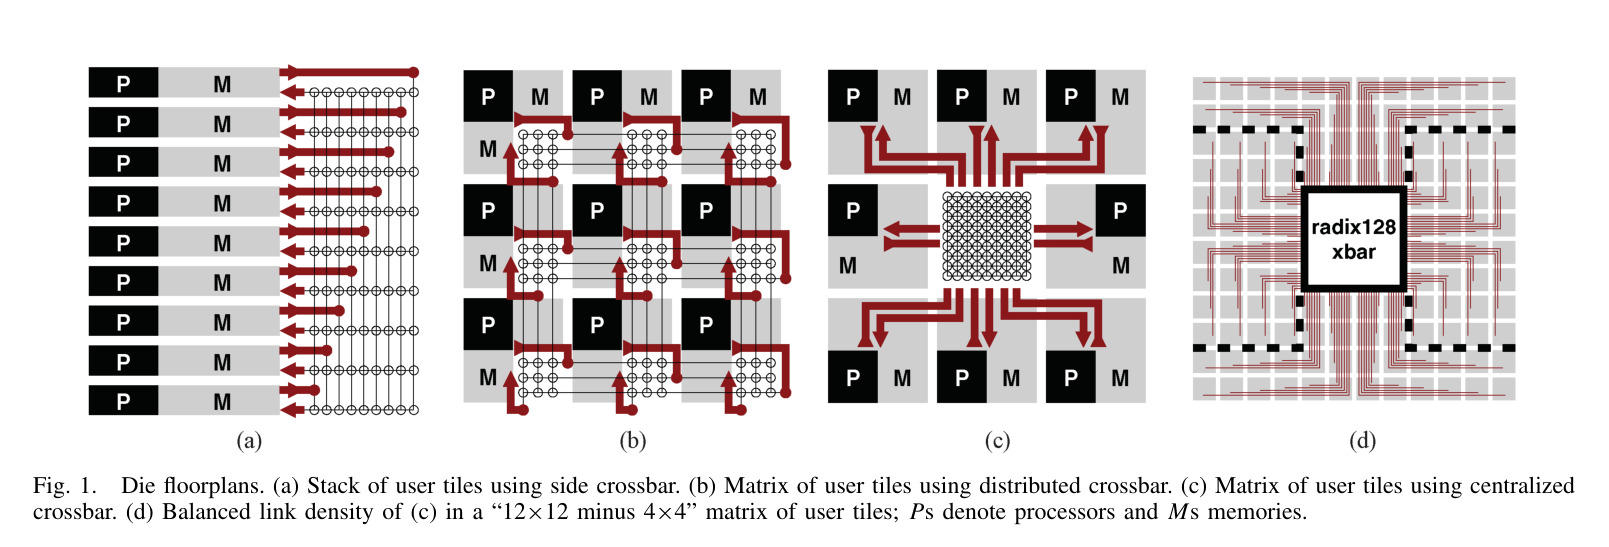
\includegraphics[width=0.88\textwidth]{chapters/ch04-topologies-and-metrics/figures/passas_fig01_crossbar_floorplans.png}
\caption{Die floorplans for crossbar-based on-chip networks. (a) Stack of user tiles with side crossbar. (b) Matrix of user tiles with distributed crossbar. (c) Centralized crossbar. (d) Balanced link density layout in a 12$\times$12 minus 4$\times$4 matrix of tiles. [Reproduced from: G. Passas, M. Katevenis, and D. Pnevmatikatos, ``Crossbar NoCs Are Scalable Beyond 100 Nodes,'' \emph{IEEE Trans. Comput.-Aided Design Integr. Circuits Syst.}, Vol.~31, No.~4, pp.~573--585, April 2012, DOI: 10.1109/TCAD.2011.2176730. \copyright~2012 IEEE]}
\label{fig:ch4_passas_floorplan}
\end{figure}

\begin{figure}[htbp]
\centering
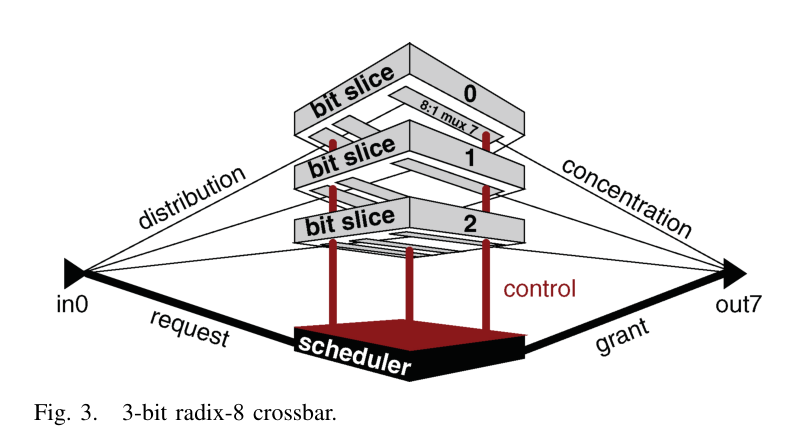
\includegraphics[width=0.65\textwidth]{chapters/ch04-topologies-and-metrics/figures/passas_fig03_radix8_crossbar.png}
\caption{Standard-cell layout of a 3-bit radix-8 crossbar bit-slice. Multiplexer circuits are routed entirely beneath upper-level metal tracks. [Reproduced from: G. Passas, M. Katevenis, and D. Pnevmatikatos, ``Crossbar NoCs Are Scalable Beyond 100 Nodes,'' \emph{IEEE Trans. Comput.-Aided Design Integr. Circuits Syst.}, Vol.~31, No.~4, pp.~573--585, April 2012, DOI: 10.1109/TCAD.2011.2176730. \copyright~2012 IEEE]}
\label{fig:ch4_passas_slice}
\end{figure}

Passas et al. proved that:
\begin{enumerate}
    \item With 8+ metal layers, crossbar wiring tracks fit directly \textbf{over standard cells} on intermediate metal layers without expanding standard-cell silicon area:
    \begin{equation}
    \text{Area}_{crossbar} \approx O(N^2 \cdot W), \quad \text{Delay}_{crossbar} \approx O(\sqrt{N \cdot W})
    \label{eq:ch4_crossbar_scaling}
    \end{equation}
    \item In a $150\text{ mm}^2$ die containing 128 $1\text{ mm}^2$ processor tiles, the radix-128 crossbar occupied **only 11\% of total die area** (including repeaters and pipeline flip-flops).
    \item Under global and stressed traffic, the monolithic crossbar delivered **up to 3$\times$ higher throughput and 2.5$\times$ lower latency** than a 2D mesh by eliminating multi-hop queueing stalls.
\end{enumerate}

\section{Quantitative Topology Evaluation Matrix}
\label{sec:ch4_summary_table}

Table~\ref{tab:ch4_metrics} summarizes the mathematical and microarchitectural metrics across major topology classes for an $N = 64$ core system.

\begin{table}[htbp]
\centering
\caption{Analytical and Empirical Metric Matrix across Interconnect Topologies ($N = 64$ nodes)}
\label{tab:ch4_metrics}
\begin{tabular}{lcccccc}
\toprule
\textbf{Topology} & \textbf{Radix ($k$)} & \textbf{Diam ($D$)} & \textbf{Avg Hops ($\bar{h}$)} & \textbf{Bisect ($B_C/W$)} & \textbf{$T_0$ (cyc)} & \textbf{Sat. Thru.} \\
\midrule
Ring (1D)                 & 2        & 32 & 16.00 & 4   & 28.00 & 0.125 \\
2D Mesh ($8 \times 8$)    & 4 (avg 3.5)& 14 & 5.33  & 16  & 12.00 & 0.500 \\
2D Torus ($8 \times 8$)   & 4        & 8  & 4.06  & 32  & 10.10 & 1.000 \\
Folded Torus ($8 \times 8$)& 4       & 8  & 4.06  & 32  & 10.10 & 1.000 \\
Hypercube (6-cube)        & 6        & 6  & 3.05  & 64  & 8.57  & 2.000 \\
Fat-Tree (3-level)        & 4        & 6  & 3.80  & 64  & 9.70  & 2.000 \\
Flattened Butterfly ($8 \times 8$) & 14 & 2 & 1.78  & 256 & 6.67  & 8.000 \\
Full Crossbar ($64 \times 64$) & 64  & 1  & 1.00  & 2048& 5.00  & 64.000 \\
\bottomrule
\end{tabular}
\end{table}

\section{Exercises and Review Questions}
\label{sec:ch4_exercises}

\begin{enumerate}
    \item \textbf{Bisection Bandwidth Bound}: Prove that under uniform random traffic, the maximum throughput per node is bounded by $\Theta \le \frac{2 B_C}{N}$. What fraction of injected traffic must traverse the bisection cut?
    \item \textbf{Folded Torus Delay}: For an $8 \times 8$ tiled chip with tile pitch $L_0 = 1.2$~mm, compare the wire delay of a naive torus wrap-around link versus a folded torus link under the Elmore delay model.
    \item \textbf{Clos Non-Blocking Sizing}: For a 3-stage Clos network $C(n, m, r)$ with $N = 64$ and $n = 8$, calculate the minimum $m$ required for strictly non-blocking operation versus rearrangeably non-blocking operation.
    \item \textbf{High-Radix Trade-Offs}: Explain why high-radix networks become more energy-efficient than low-radix 2D meshes as core counts scale beyond 100 nodes.
\end{enumerate}
